
\section*{Lecture 3, Step-Indexing}
This lecture was on extending the unary logical relation for type safety of simply typed lambda calculus to recursive types, introducing universal types, and finally a short introduction to contextual equivalence.

\subsection*{Simply typed lambda calculus extended with $\mu$}
In a naive first attempt to make the value interpretation we could write something like
\[
  \vpred{\mu\alpha. \; \tau} = \{\fold \; v \vbar \unfold \; (\fold \; v) \in \epred{\sub{\tau}{\mu\alpha.\;\tau}{\alpha}} \}
\]
We can simplify this slightly; first we use the fact that $\unfold \; (\fold \; v)$ reduces to $v$. Next, we use the fact that $v$ must be a value and the fact that we want $v$ to be in the expression interpretation of $\tau[\mu \alpha. \; \tau / \alpha]$. By unfolding the definition of the expression interpretation we conclude that it suffices to require $v$ to be in the value interpretation of the same type. We then end up with the following definition:
\[
  \vpred{\mu\alpha. \; \tau} = \{\fold \; v \vbar v \in \vpred{\sub{\tau}{\mu\alpha.\;\tau}{\alpha}} \}
\]
This gives us a well-foundness issue. The value interpretation is defined by induction on the type, $\sub{\tau}{\mu\alpha.\;\tau}{\alpha}$ is not a structurally smaller type than $\mu\alpha. \; \tau$. 

To solve this issue we index the interpretation by a natural number which we write as follows:
\[
  \vpres{\tau} = \{v \vbar \dots \}
\]
If $v$ belongs to the interpretation, then this is read as ``$v$ belongs to the interpretation of $\tau$ for $k$ steps.'' We interpret this in the following way; given a value that we run run for $k$ or fewer steps as in the value is used in some program context for $k$ or fewer steps, then we will never notice that it does not have type $\tau$. If we use the same value in a program context that wants to run for more than $k$ steps, then we might notice that it does not have type $\tau$ which means that we might get stuck. This gives us an approximate guarantee.

We use this as an inductive metric to make our definition well-founded, so we define the interpretation on induction on the step-index followed by inner induction on the type structure. Let us start by adding the step-index to our existing value interpretation:
\begin{align*}
  \vpres{bool} &= \{\true,\false\} \\
  \vpres{\tarrow{\tau_1}{\tau_2}} &= \{\tlabs{x}{\tau_1}{e} \vbar \forall j \leq k. \; \forall v \in \vpres[j]{\tau_1}. \; \sub{e}{v}{x} \in \epres[j]{\tau_2} \}
\end{align*}
$\true$ and $\false$ are in the value interpretation of $bool$ for any $k$, so $\true$ and $\false$ will for any $k$ look like it has type $bool$. To illustrate how to understand the value interpretation of $\tarrow{\tau_1}{\tau_2}$ please consider the following timeline:  \\
\begin{center}
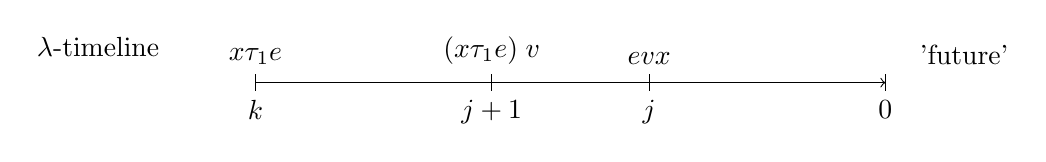
\begin{tikzpicture}
    % draw horizontal line   
    \draw[->] (0,0) -- (8,0);

    % draw vertical lines
    \foreach \x in {0,3,5,8}
      \draw (\x cm,3pt) -- (\x cm,-3pt);

    % draw nodes
    \draw (-2,0) node[below=3pt] {  } node[above=6pt] {$\lambda$-timeline};
    \draw (0,0) node[below=3pt] {$k$} node[above=3pt] {$ \tlabs{x}{\tau_1}{e}$};
    \draw (3,0) node[below=3pt] {$ j+1 $} node[above=3pt] {$(\tlabs{x}{\tau_1}{e})\; v $};
    \draw (4.3,0) node[below=3pt] {$   $} node[above=3pt] {$ \evalto $};    
    \draw (5,0) node[below=3pt] {$ j $} node[above=3pt] {$ \sub{e}{v}{x} $};
    \draw (8,0) node[below=3pt] {$ 0 $} node[above=3pt] {$  $};
    \draw (9,0) node[below=3pt] {$   $} node[above=3pt] { 'future' };
  \end{tikzpicture}
\end{center}
Here we start at index $k$ and as we run the program we use up steps until we at some point reach 0 and rund out of steps. At step $k$ we are looking at a lambda. A lambda is used by applying it, but it is not certain that the application will happen right away, as the we only do $\beta$-reduction when we try to apply a lambda to a value, but we might be looking at a context where we want to apply the lambda to an expressions, i.e.\ $(\tlabs{x}{\tau_1}{e})\; e_2$. We might use a bunch of steps to reduce $e_2$ down to a value, but we cannot say how many. So say that sometime in the futurewe have fully evaluated $e_2$ to $v$ and say that we have $j+1$ steps left at this time, then we can do the $\beta$ reduction which gives us $\sub{e}{v}{x}$ at step $j$. % If we ever hit 0 steps, then all bets are off. the value can have any type.

We can now define the value interpretation of $\mu\alpha. \; \tau$:
\[
  \vpres{\mu\alpha.\; \tau} = \{\fold \; v \vbar \forall j < k. \; v \in \vpres[j]{\tau\sub{\mu\alpha.\;\tau}{\alpha}} \}
\]
This definition is like the one we previously proposed, but with a step-index. This definition is well-founded because $j$ is required to be \emph{strictly} less than $k$ and as we define the interpretation on induction over the step-index this is indeed well founded. We do not define a value interpretation for type variables $\alpha$, as we have no polymorphism yet. The only place we have a type variable at the moment is in $\mu\alpha. \; \tau$, but in the interpretation we close of the $\tau$ under the $\mu$, so we will never encounter a free type variable.

Finally, we define the expression interpretation:
\[
  \epres{\tau} = \{e \vbar \forall j < k. \; \forall e'. \; e \evaltos[j] e' \; \wedge \; \irred(e') \; \implies \; e' \in \vpres[k-j]{\tau}\}
\]
To illustrate what is going on here consider the following timeline: \\
\begin{center}
\begin{tikzpicture}
    % draw horizontal line   
    \draw[->] (0,0) -- (4,0);

    % draw vertical lines
    \foreach \x in {0,2,4}
      \draw (\x cm,3pt) -- (\x cm,-3pt);

    % draw nodes
    \draw (0,0) node[below=3pt] {$k$} node[above=3pt] {$e$};
    \draw (1,0) node[below=3pt] {$ $} node[above=3pt] {$\evalto \evalto \evalto \evalto$};
    \draw (2,0) node[below=3pt] {$k-j$} node[above=3pt] {$e'$};
    \draw (4,0) node[below=3pt] {$0$} node[above=3pt] {$  $};

    % brace
    \draw [decorate,decoration={brace,amplitude=10pt,mirror}]
    (0,-0.6) -- (2,-0.6) node [black,midway,yshift=-0.5cm] 
          {\footnotesize $j$};
\end{tikzpicture}
\end{center}
We start with an expression $e$, then we take $j$ steps and get to expression $e'$. At this point if $e'$ is irreducable, then we want it to belong to the value interpretation of $\tau$ for $j-k$ steps. The reason we use a strict inequality is that we do not want to hit 0 steps. If we hit 0 steps, then all bets are off.%TODO: why are all bets off?

We also need to lift the interpretation of type environments to step-indexing:
\begin{align*}
  \gpres{\mtenv} & = \{\emptyset \} \\
  \gpres{\Gamma, x : \tau} & = \{ \gamma[x \mapsto v] \vbar \gamma \in \gpres{\Gamma} \; \wedge \; v \in \vpres{\tau} \}
\end{align*}

\[
  \Gamma \models e : \tau \eqdef \forall k \geq 0. \; \forall \gamma \in \gpres{\Gamma} \; \implies \gamma(e) \in \epres{\tau}
\]

\begin{stlcmufundprop}[Fundemental property]
  If $\Gamma \vdash e : \tau$ then $\Gamma \models e : \tau$.
\end{stlcmufundprop}

\[
\circled{b} \quad \mtenv \models e : \tau \implies \safe(e)
\]

\begin{monotonicity}
  If $v\in \vpres{\tau}$ and $j \leq k$  then $v \in \vpres[j]{\tau}$.
\end{monotonicity}
\begin{proof}
We prove this by case on $\tau$.
\case{$\tau = bool$}
assume $v \in \vpres{bool}$ and $j \leq k$, we then need to show $v \in \vpres[j]{bool}$. As $v \in \vpres{bool}$ we know that either $v= \true$ or $v=\false$. If we assume $v=\true$, then we immidiately get what we want to show, as $\true$ is in $\vpres[j]{bool}$ for any $j$. Likewise for the case $v=\false$.
\case{$\tau = \tarrow{\tau_1}{\tau_2}$}
assume $v \in \vpres{\tarrow{\tau_1}{\tau_2}}$ and $j \leq k$, we then need to show $v \in \vpres[j]{\tarrow{\tau_1}{\tau_2}}$. As $v$ is a member of $\vpres{\tarrow{\tau_1}{\tau_2}}$ we can conclude that $v = \tlabs{x}{\tau_1}{e}$ for some $e$. By definition of $v \in \vpres[j]{\tarrow{\tau_1}{\tau_2}}$ we need to show $\forall i \leq j. \forall v' \in \vpres[i]{\tau_1}.\; v' \in \epres[i]{\tau_2}$. Suppose $i \leq j$ and $v' \in \vpres[i]{\tau_1}$, we then need to show $v' \in \epres[i]{\tau_2}$.

By assumption we have $v \in \vpres{\tarrow{\tau_1}{\tau_2}}$ which gives us $\forall n \leq k. \forall v' \in \vpres[n]{\tau_1}.\; v' \in \epres[n]{\tau_2}$. From $j \leq k$ and $i \leq j$ we get $i \leq k$ by transitivity. We use this with $v' \in \vpres[i]{\tau_1}$ to get $v' \in \epres[i]{\tau_2}$ which is what we needed to show.
\case{$\tau = \mu \alpha.\; x$}
assume $v \in \vpres{\mu\alpha. \; \tau}$ and $j \leq k$, we then need to show $v \in \vpres[j]{\mu\alpha. \; \tau}$. From $v$'s assumed membership of the value interpretation of $\tau$ for $k$ steps we conclude that there must exist a $v'$ sucht that $v = \fold \; v'$. If we suppose $i<j$, then we need to show $v' \in \vpres[i]{\subst{\tau}{\mu\alpha.\; \tau}{\alpha}}$. From $i<j$ and $j \leq k$ we can conclude $i < k$ which we use with $\forall n < k.\; v' \in \vpres[n]{\subst{\tau}{\mu\alpha.\; \tau}{\alpha}}$, which we get from $v \in \vpres{\mu\alpha. \; \tau}$, to get $v' \in \vpres[i]{\subst{\tau}{\mu\alpha.\; \tau}{\alpha}}$.
\end{proof}

\begin{proof}[Proof (Fundemental Property)]
  
\end{proof}

\[
  \vpres{\tau_1 + \tau_2} = \{\inl \; v_1 \vbar v_1 \in \vpres{\tau_1}\} \cup 
                            \{\inr \; v_2 \vbar v_2 \in \vpres{\tau_2}\}
\]

\subsection*{Universal Types}
\[
  sort \; : \; \forall \alpha.\; \tarrow{(list \; \alpha) \times (\tarrow{\alpha \time \alpha}{bool} )}{list \; \alpha}
\]
\[
  sort[int](3,5,7)<
\]
\[
  \tLabs{e}
\]

\subsubsection*{System F (Simply Typed Lambda Calculus With Universal Types)}
\begin{align*}
  \tau &::= \dots \vbar \forall \alpha. \; \tau \\
  e    &::= \dots \vbar \tLabs{e} \vbar e[\tau] \\
  v    &::= \dots \vbar \tLabs{e}\\
  E    &::= \dots \vbar \fold \; E[\tau] 
\end{align*}
\[
  (\tLabs{e}[\tau]) \evalto e[\tau/\alpha]
\]
Type environment
\[
  \Delta ::= \mtenv \vbar \Delta,\; \alpha
\]
Type judegement form:
\[
  \Delta,\Gamma \vdash e : \tau
\]
Well formed type:
\[
  \Delta \vdash \tau \eqdef \FTV(\tau) \subseteq \Delta
\]
where $\FTV(\tau)$ is the set of free type variables in $\tau$.

Well-formed environment
\[
  \Delta \vdash \Gamma \eqdef \forall x \in \dom(\Gamma). \; \Delta \vdash \Gamma(x)
\]
For any type judgement $\Delta,\Gamma \vdash e : \tau$ we have as an invariant that $\Delta \vdash \Gamma$.
Typing rules:
\[
  \FTFalse
\hspace{1cm}
  \FTTrue
\]
\[
  \FTVar
\hspace{1cm}
  \FTIf
\]  
\[
  \FTAbs 
\hspace{1cm}
  \FTApp
\]

\begin{theorem}
  If $\mtenv ; \mtenv \vdash e : \forall \alpha. \; \tarrow{\alpha}{\alpha}$,\\ $\mtenv \vdash \tau$, and\\ $\mtenv; \mtenv \vdash v : \tau$\\ then $e[\tau]\; v \evaltos v$
\end{theorem}

\subsection*{Exercises}
\begin{enumerate}
\item Do the lambda and application case of the \emph{Fundemental Property} theorem.%Specify in what proof, probably fundemental property
\item Try to prove the monotonicity lemma where the definition of the value interpretation has been adjusted with:
\[
\vpres{\tarrow{\tau_1}{\tau_2}} = \{\tlabs{x}{\tau_1}{e} \vbar \; \forall v \in \vpres{\tau_1}. \; \sub{e}{v}{x} \in \epres{\tau_2} \}
\]
This will fail, but it is instructive to see how it fails.
\end{enumerate}


%induction on step index followed by inner induction on the type structure.
%when an expression looks like it has type tau.
\clearpage
